\chapter{Bayesian Clustering of Student Solutions}\label{chapter:grovercode}

The original vision of OverCode was to discover pedagogically valuable themes of variation within thousands of student solutions to the same programming problem. While OverCode does normalize and cluster correct solutions so that they can be more easily understood as a group, it does not pull out larger themes of variation as clearly as initially hoped.

%\section{Clustering Solutions with Statistical Models}\label{sec:latent}

%One approach to pulling out larger themes of variation within solutions is to cluster more aggressively. 

The current OverCode pipeline performs deterministic interpretable unsupervised clustering in order to produce stacks of similar solutions. What can vary and what is invariant across all the solutions within a stack is clear, just by reading the platonic solution that represents the stack. Syntactic differences split apart groups of solutions into smaller stacks so that each stack's platonic solution matches the syntax used in the solutions in represents. This can also produce more stacks than teachers can read.% In the interface, the human can step in and indicate which syntactic differences they do not care about, but  %Only in the interface can a human step in and tell the system to ignore certain syntactic differences.

%There are several promising methods that may help merge stacks in future versions of the OverCode pipeline. 

%Once a set of semantically equivalent and probabististically semantically equivalent could be used to identify semantically equivalent subexpressions across many solutions

%Probablistic semantic equalivalence (PSE)~\cite{codewebs} is a similar concept applied to subexpressions. Overcode renames variables to their most common name across all solutions. OverCode could, in the future, also replace PSE subexpressions with their most common form across all solutions.

%OverCode already uses its own form of probablistic semantic equality (PSE)~\cite{codewebs}, i.e., equality with respect to a test suite, to normalize variable names. This can be extended to subexpressions as well. Overcode renames PSE variables to their most common name across all solutions. OverCode could also replace PSE subespressions with their most common form across all solutions.

%Compiler optimizations could be used to merge OverCode clusters. However, as a system designer, one must decide or give the teacher control over how many different, semantically equivalent solutions are collapsed into a single cluster since. %These methods are discussed again in the future work, because the second set of methods were chosen for future investigation in this chapter.

OverCode's normalized stacks exhibit statistical regularity. Given that variation theory is interested in dimensions of variation and consistency that characterize all possible instantiations of an idea, statistical methods warrant further investigation. Latent variable models are a type of statistical model that attempt to explain variation in a dataset based on underlying factors. With the right choice of features and model, a latent variable model may be able to capture underlying design choices. In this section, two latent variable models have been explored in a preliminary way for this purpose: the Bayesian Case Model (BCM)~\cite{} and Latent Dirichlet Allocation (LDA)~\cite{}. 

BCM was selected because, like the original OverCode pipeline, it clusters solutions and produces a single solution to represent the entire cluster. Like OverCode, it also indicates the features that characterize each cluster. While OverCode displays the platonic solution that shares the same set of normalized lines with all other members of the cluster, BCM learns a subspace of features that it determines are most characteristic of the solutions within that cluster. 

BCM has an interactive variant called iBCM. iBCM allows the teacher to directly modify the prototype and the subspace chosen by BCM if it disagrees with their domain knowledge or preferences. This teacher action triggers a rerun of BCM with the modifications taken into account.%is taken into account by the algorithm 

Internally, BCM depends on a mixture model with a Dirichlet prior. Rather than find a cluster for each entire solution, mixture models can learn clusters of features that co-exist across some subset of all solutions. The concentration parameter of the BCM Dirichlet prior is set to promote sparsity, i.e., mixture distributions over solutions that have the majority of their probability mass on a single mixture component. BCM then assigns each solution to a cluster according to its most probable mixture component. %In other words, after fitting the model to the data, each solution will likely have a single dominant mixture component associated with it. If data points were documents instead of solutions, one would say that each document is determined to have a single dominating topic.

Since teachers can be poor at clustering solutions, i.e., inconsistent with each other~\cite{berkeleymastersthesis}, it may also be difficult for any algorithm to find a clustering that appeals to most teachers. However, there are a statistical models, lie LDA, that cluster components of solutions instead of entire solutions. LDA was selected as an alternative to BCM in order to explore how solution component clustering might better support teachers who do not agree on whole-solution clusterings.

%LDA clusters components of solutions, rather than assigning entire solutions to a particular cluster. This is an appealing model choice . % or even deciding which solutions are more similar to each other than others~\cite{}. 

BCM was built explicitly with interpretability in mind, but it is still not clear whether LDA or BCM are more interpretable in the context of clustering OverCode stacks. LDA has some known interpretability problems. As part of its training process, LDA learns distributions over features, also known as {\it mixture components}. It can be difficult to interpret exactly what an LDA mixture component means just by looking at its distribution over features.

%and distributions of those mixtures over each solution in the set it is trained on. 

%However, sorting solutions based on the degree to which a particular topic is associated with them may pull out a distinctive, human-interpretable themes. 

%Furthermore, when using LDA, the concentration parameter of the Dirichlet prior need not promote for sparsity; it can be tuned by a human or a heuristic, to maximize the usefulness of the resulting breakdown into mixture components. This parameter's optimal value may be problem-specific and teacher-specific. 



\subsection{Clustering Solutions with BCM}

BCM was applied to the platonic solutions generated by OverCode. The platonic solutions encode both static and dynamic information, i.e., the syntax carries the static information and the variable naming encodes dynamic information. The platonic solution is tokenized and represented as a binary vector indicating the existence of the features, including renamed variables and language-specific keywords, such as normalized variable names like \texttt{listA} and Python keywords like \texttt{assert} and \texttt{while}. The result is a clustering of OverCode platonic solutions. 

BCM was run on three different programming problems selected from those previously analyzed in Chapter~\ref{chapter:overcode}. An interface, shown in Figure~\ref{overcode_ibcm}, displayed the results, with iBCM continuing to run in the backend, ready to update the clustering in response to teacher feedback. The interface afforded promoting a member of a cluster to be its prototype and clicking on a token within a prototype, such as a variable name or keyword, to toggle whether or not it is labeled a characteristic feature of that cluster.

In order to determine whether or not these clusterings and interface affordances are useful to teachers, a small pilot study was run on three teachers of introductory Python programming. For the pilot, two more interfaces were introduced as controls. One is a duplicate of the control interface used in the OverCode studies, i.e., a long list of syntax highlighted raw solutions in a random order in the browser. The second interface differs from the previous control by one factor: the raw solutions are replaced with their platonic equivalents.

The teachers were each given sets of Python solutions to view in each of the three interfaces. For each problem, they were asked to create a grading rubric and provide helpful comments for the students of the type that might be mentioned in a class-wide forum post.

%, based on interacting with solutions in one of three different interfaces. The three interfaces were: (1) raw solutions in the browser, similar to the control used in the OverCode studies, (2) the OverCode platonic solutions, and (3) a BCM clustering of OverCode clusters, i.e., the prototypes and characteristic features of each BCM cluster, as well as its cluster members. 

 %Both these modifications triggered BCM running in the backend to rerun and send a new clustering to the front end for display. 

Pilot users appreciated the fact that BCM gave some structure to the space of solutions. Rather than a long list of solutions, the interface suggested distinct subpopulations of solutions within the list. However, subjects did not fully understand the probabilistic nature of the clustering method. The presence of a single intruder, i.e., a solution that the teacher believed did not belong in a cluster, caused confusion. This could be ameliorated by giving teachers more ways to modify the clustering, e.g., allowing teachers the option to kick an intruder out of a cluster and rerun BCM, or by introducing the tool as a mechanism for discovery instead of organization. Subjects also requested richer or higher-level features than variable names and keywords. Been Kim's PhD thesis~\cite{beenthesis} describes a follow-up full user study comparing the efficacy of BCM and iBCM on clustering OverCode platonic solutions.

\begin{figure}[ht]
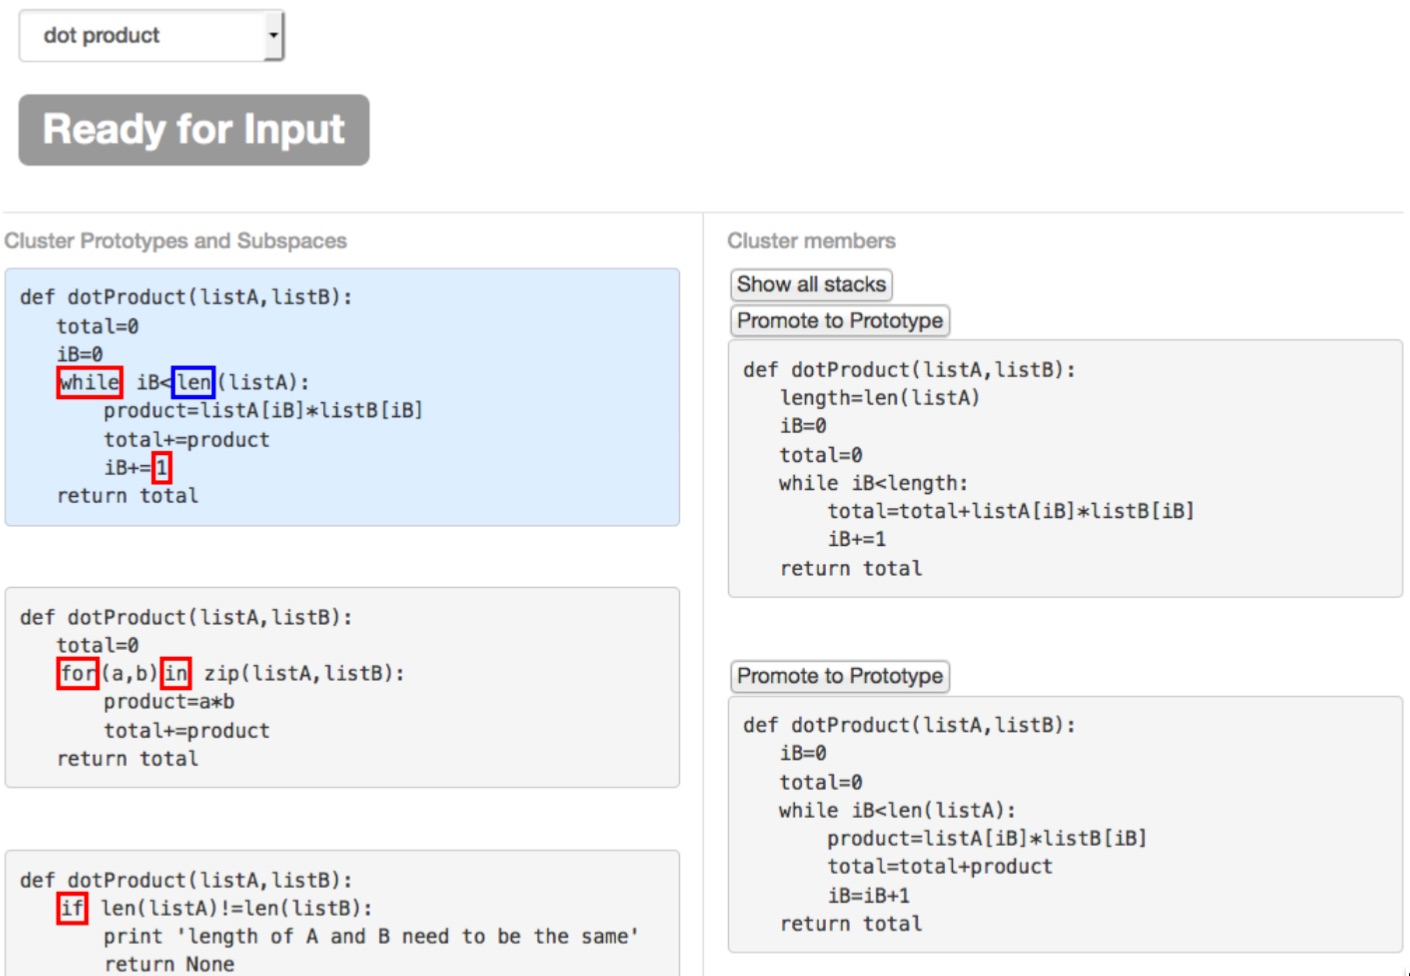
\includegraphics[width=0.75\columnwidth]{Body/figures/grovercode/overcode_ibcm}
\caption{The solutions on the left are cluster prototypes. The blue solution is the selected cluster whose members are shown in a scrollable list on the right-hand side. The tokens contained in red boxes are features that BCM identifies as characteristic of the cluster represented by that prototype. When a user hovers their cursor over a keyword or variable name, e.g., \texttt{len}, it is highlighted in a blue rectangle, indicating that it can be interacted with, i.e., clicked.}
\label{overcode_ibcm}
\end{figure} 

\subsection{Clustering Solution Components with LDA}

Other researchers have documented a lack of agreement across human-made clusters of student solutions~\cite{berkeleymastersthesis}. One possible explanation for poor consistency is that solutions are mixtures of design choices and teachers care differently about various aspects of solutions. If student A writes a solution with a well-written loop and extraneous statements while student B writes a solution with extra loops but otherwise very clean code, teachers can reasonably disagree about which cluster each whole solution should be placed in, depending on whether they believe inefficient control flow or extraneous statements are worse.

Instead of trying to approximate clusterings that humans do not even agree on, it may be more useful to model solutions as mixtures of good and bad design choices. While more sophisticated mixture models' assumptions may ultimately be more appropriate, LDA \cite{lda} as implemented in the Gensim toolbox \cite{gensim} was chosen as the model to evaluate in this preliminary work. 

Like BCM, LDA was run on the platonic solutions. However, the representation of these solutions was also changed: in order to pull out higher-level patterns in approach, rather than lower-level patterns in syntax, solutions were represented solely by the behavior of the variables within them. 

As described in the chapter on OverCode, the OverCode analysis pipeline executes all programs on a common set of test cases and records the sequence of values taken on by each variable in the program. OverCode assumes that variables in different programs that transition through the same sequence of values on the same test cases are in fact fulfilling the same semantic role in the program. %This sequence of values taken on by each variable in each program becomes a signature, i.e., the key to recognizing semantically equivalent variables across programs.  % and can therefore be considered the same {\bf common variable} uniquely defined by that sequence of values.



\begin{figure}[ht]
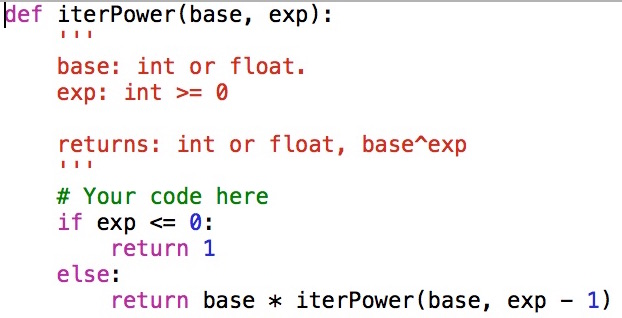
\includegraphics[width=0.75\columnwidth]{Body/figures/grovercode/recursive_example}
\caption{Example of a recursive student solution.}
\label{recursive_example}
\vspace*{\floatsep}
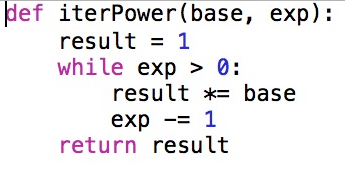
\includegraphics[width=0.45\columnwidth]{Body/figures/grovercode/whilestandard}
\caption{Example of a student solution using the Python keyword \texttt{while}.}
\label{whilestandard}
\vspace*{\floatsep}
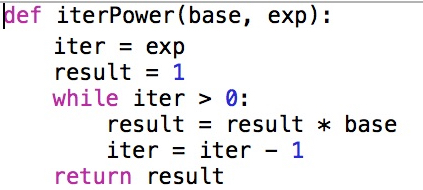
\includegraphics[width=0.5\columnwidth]{Body/figures/grovercode/augmentedwhile}
\caption{Example of a student solution using the Python keyword \texttt{while}, where the student has not modified any input arguments, i.e., better programming style.}
\label{augmentedwhile}
\end{figure} 

Below are the sequences of variable values recorded by OverCode while executing \texttt{iterPower(5,3)} as defined in Figures \ref{recursive_example}, \ref{whilestandard}, and \ref{augmentedwhile}:
\begin{itemize}
  \item {\bf Figure \ref{recursive_example}}
  \begin{itemize}
  \setlength\itemsep{0.05em}
  \item \texttt{exp: 3, 2, 1, 0, 1, 2, 3}
  \item \texttt{base: 5}
  \end{itemize}
  \item {\bf Figure \ref{whilestandard}}
  \begin{itemize}
  \item \texttt{exp: 3, 2, 1, 0}
  \item \texttt{base: 5}
  \item \texttt{result: 1, 5, 25, 125}
  \end{itemize}
  \item {\bf Figure \ref{augmentedwhile}}
  \begin{itemize}
  \item \texttt{exp: 3}
  \item \texttt{base: 5}
  \item \texttt{iter: 3, 2, 1, 0}
  \item \texttt{result: 1, 5, 25, 125}
  \end{itemize}
\end{itemize}

In the previous examples, the input argument \texttt{base} would be considered variable common to all three programs, but the input argument \texttt{exp} would not be. The variable \texttt{result} would also be considered a common variable shared across just the definitions in Figure \ref{whilestandard} and Figure \ref{augmentedwhile}. This allows us to distinguish between programs that calculate the answer in semantically distinct ways, without discriminating between the low-level design decisions about syntax. 

LDA is often applied to corpora of textual documents, where the corpus is represented as a $W \times N$ term-by-document matrix of counts, where $W$ is the vocabulary size across all documents and $N$ is the number of documents. In this representation, the document is represented a bag of word counts, i.e., how many times each word appears in the document. Following this analogy, solutions are represented as a bag of variable behaviors. The matrix representing the solutions in Figures \ref{recursive_example} through \ref{augmentedwhile} executed on \texttt{iterPower(5,3)} is shown in Table \ref{varbydocmat}.

\begin{table}[t]
\caption{Variable-by-Solution Matrix for Programs, where variables are uniquely identified by their sequence of values while run on a set of test case(s)}
\label{varbydocmat}
%\vskip 0.15in
\begin{center}
\begin{small}
\begin{sc}
\begin{tabular}{| l | c | c | c | c | c |}
\hline
%\abovespace\belowspace
Sol- & \texttt{5} & \texttt{1,5,...} & \texttt{3,2,1,0,} & \texttt{3,2,1,0} & \texttt{3} \\
ution& & \texttt{25,125} & \texttt{...1,2,3} & &  \\
\hline
%\abovespace
Figure \ref{recursive_example} & 1 & 0 & 1 & 0 & 0 \\
Figure \ref{whilestandard}     & 1 & 1 & 0 & 1 & 0 \\
Figure \ref{augmentedwhile}    & 1 & 1 & 0 & 1 & 1 \\
\hline
\end{tabular}
\end{sc}
\end{small}
\end{center}
%\vskip -0.1in
\end{table}

Note that, while the entries in Table \ref{varbydocmat} only take on values $0$ or $1$, more complicated definitions may have $n$ instances of, e.g., a variable that takes on the sequence of values \texttt{3,2,1,0}. In that case, there could be an $n$ in the \texttt{3,2,1,0} column for the row corresponding to that solution, or it can be left as a binary indicator. %In other words, true to the assumptions made by LDA, these are occurrence counts, not binary indicators.

%\subsection{Procedure}

In order to run LDA, 3875 student solutions to \texttt{iterPower} were first run on a set of test cases within the OverCode analysis pipeline. The OverCode pipeline produced a set of 977 platonic solutions and a set of features for each solution, including which variable sequences were observed during execution. Another script turned this output into a variable-by-solution matrix for the 977 platonic solutions, which were then fed into LDA for analysis. LDA was run repeatedly with multiple values for the parameter that sets the number of latent mixture components. The results were examined by hand since perplexity and held-out likelihoods are not necessarily good proxies for human interpretability \cite{readingtealeaves}. 

Since the learned mixture components are distributions over variable behaviors, it is easier to inspect solutions which have high amounts of that mixture component within them and infer a theme by comparing them to solutions that contain high amounts of a different mixture component. These comparisons were done by hand for a subset of popular mixture components for each LDA model. One topic comparison captured the difference between solutions like Figure ~\ref{augmentedwhile} and ~\ref{whilestandard}. Another topic comparison exposed the difference between the subpopulation of solutions with extra (unnecessary) conditional statements and the common, more concise solution. In the future, a user interface would be very helpful for this task, especially one which made it easier to compare the output of models with different parameter values. 

LDA applied to a variable-by-solution matrix is a promising method for identifying variation within corpora of solutions to the same programming problem. However, the assumptions made in LDA, such as the independence of mixture components, and requirements, such as explicitly setting the number of mixture components beforehand, may mean that other mixture models, such as the Correlated Topic Model~\cite{}\todo{fill in} or the Hierarchical Dirichlet Process~\cite{}\todo{fill in} will ultimately be a better model fit for this purpose.



\section{Conclusion}
The clustering described in the original OverCode work was relatively limited in scope, but it did produce platonic solutions that can be used for more statistically sophisticated clustering techniques and as a starting point for helping graders understand and grade incorrect student solutions by hand.

